%%%%%%%%%%%%%%%%%%%%%%%%%%%%%%%%%%%%%%%%%%%%%%%%%%%%%%%%%%%%%%%%%%%%%%%%%%%%%%%%%%
\begin{frame}[fragile]\frametitle{}
\begin{center}
{\Large Introduction}
\end{center}
\end{frame}


%%%%%%%%%%%%%%%%%%%%%%%%%%%%%%%%%%%%%%%%%%%%%%%%%%%
\begin{frame}[fragile] \frametitle{What is Deep Learning?}

\begin{itemize}
\item Artificial Intelligence: mimicking human intelligence
\item Machine Learning: Automating Learning with features. 
\item ML: human-designed representations and input features.  So, its just optimizing weights to best make a final prediction
\item There could be programmed (hand coded) AI, that's not Machine Learning
\item Machine Learning could be for non AI activities, like automation
\item Deep Learning: Neural network with no input features
\end{itemize}
\end{frame}


%%%%%%%%%%%%%%%%%%%%%%%%%%%%%%%%%%%%%%%%%%%%%%%%%%%%%%%%%%
\begin{frame}[fragile] \frametitle{ML vs DL: What's the difference?}
\begin{center}
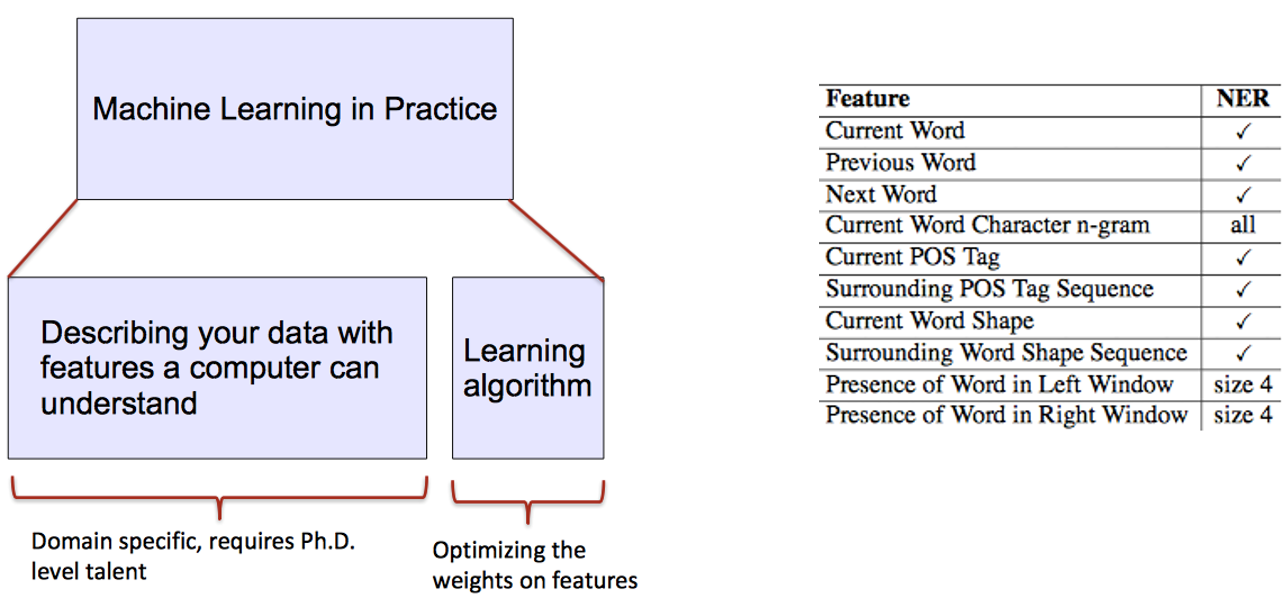
\includegraphics[width=\linewidth,keepaspectratio]{dlfeat}
\end{center}
\tiny{(Reference: Introduction to Deep Learning - Ismini Lourentzou)}
\end{frame}



%%%%%%%%%%%%%%%%%%%%%%%%%%%%%%%%%%%%%%%%%%%%%%%%%%%
\begin{frame}[fragile] \frametitle{ML vs DL: What's the difference?}
Deep learning algorithms attempt to learn (multiple levels of) representation by using a hierarchy of multiple layers
\begin{center}
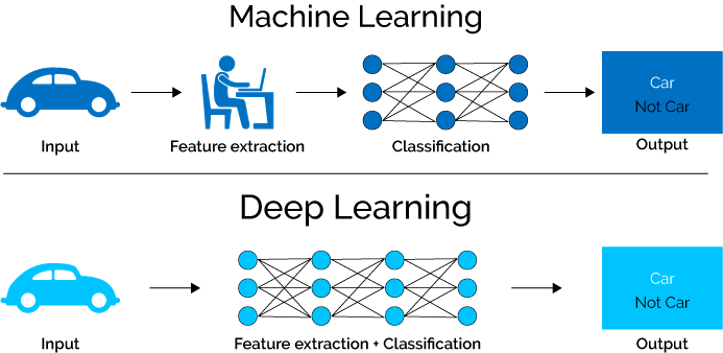
\includegraphics[width=\linewidth,keepaspectratio]{dlfeat1}
\end{center}
\tiny{(Reference: https://www.xenonstack.com/blog/static/public/uploads/media/machine-learning-vs-deep-learning.png)}

\end{frame}

%%%%%%%%%%%%%%%%%%%%%%%%%%%%%%%%%%%%%%%%%%%%%%%%%%%%%%%%%%
\begin{frame}[fragile] \frametitle{AI ML DL: What's the difference?}
\begin{center}
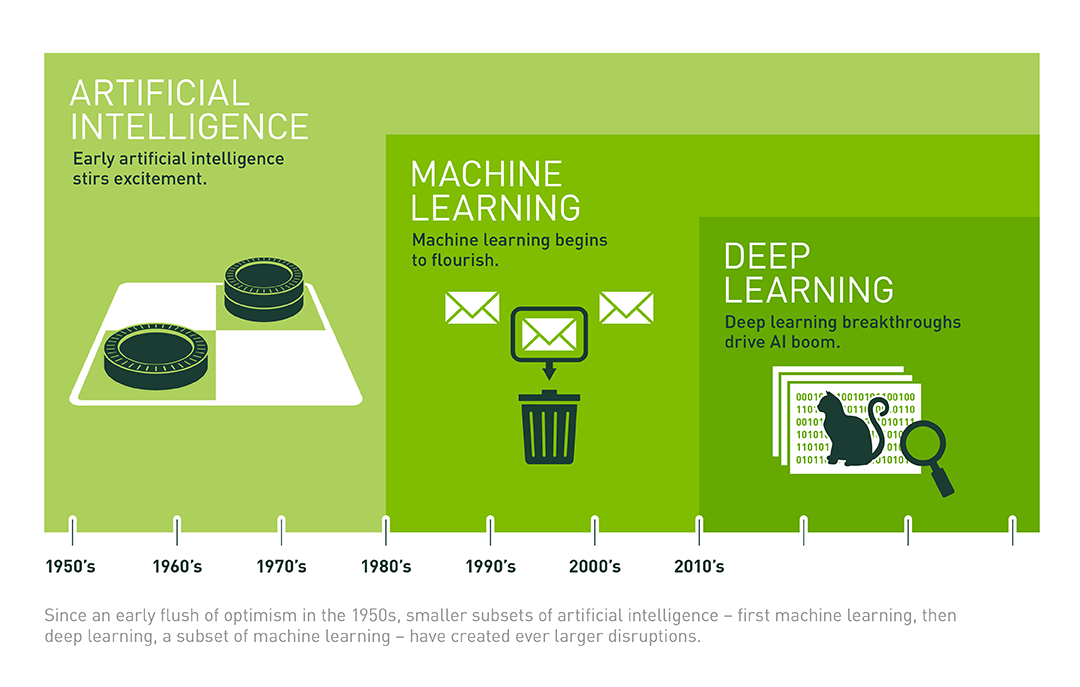
\includegraphics[width=\linewidth,keepaspectratio]{aimldl}
\end{center}

\tiny{(Reference: The Difference Between AI, Machine Learning, and Deep Learning - NVIDIA Blog)}
\end{frame}


%%%%%%%%%%%%%%%%%%%%%%%%%%%%%%%%%%%%%%%%%%%%%%%%%%%%%%%%%%
\begin{frame}[fragile] \frametitle{History}
\begin{center}
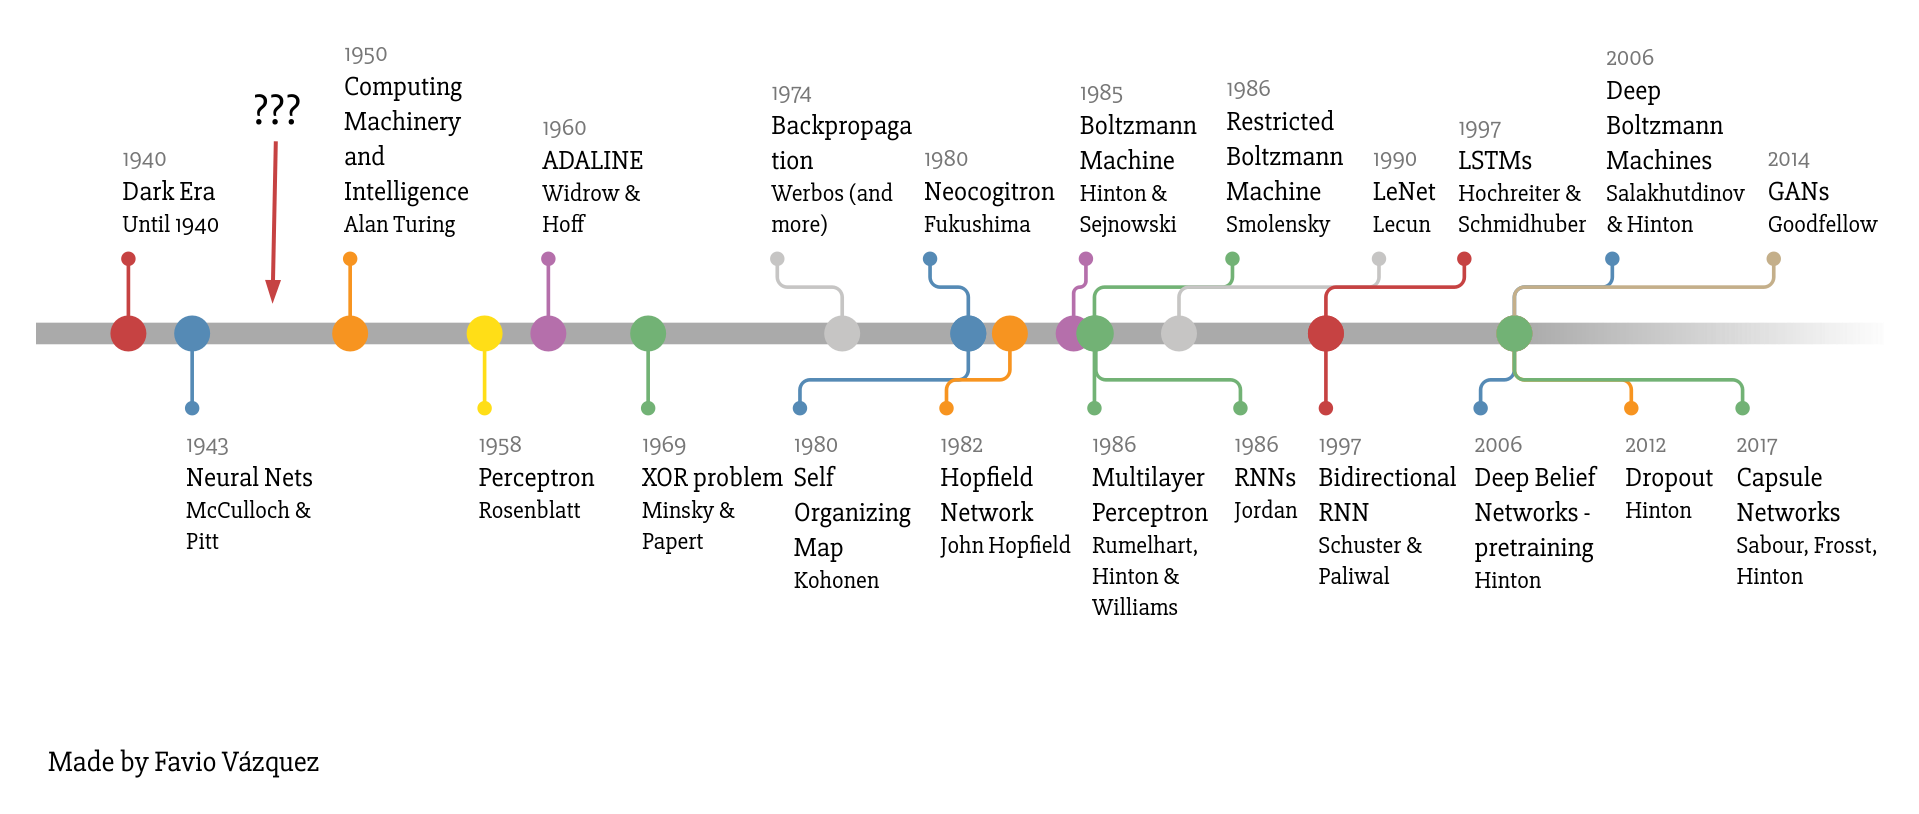
\includegraphics[width=\linewidth,keepaspectratio]{dl_timeline}
\end{center}

\tiny{(Reference: Deep Learning basics - Rodrigo Agundez)}
\end{frame}

%%%%%%%%%%%%%%%%%%%%%%%%%%%%%%%%%%%%%%%%%%%%%%%%%%%
\begin{frame}[fragile] \frametitle{History}
\begin{itemize}
\item  1958 - Percentron unit - Frank Rosenblatt
\item  1986 - Backpropagation - Geoffrey Hinton
\item 1986 - RNN - Schuster \& Pallwal
\item  1989 - LeNet Backpropagation to multi-layer perceptron - Yan LeCun
\item 1997 - LSTM - Sepp Hochreiter and Jürgen Schmidhuber
\item  1998 - LeNet-5 Convolutional neural networks - YanLecun
\item  2007 - Fei Fei Li Princeton ImageNet competition
\item  2009 - GPU for deep learning - Andrew Ng
\item  2011 - Demonstration of ReLu for deep neural networks - Yoshua Bengio
\item  2012 - AlexNet wins ImageNet 25\% to 16\% error
\item  2012 - Dropout technique - Geoffrey Hinton
\item  2014 - Generative adversarial networks - Ian Goodfellow \& Yoshua Bengio
\item  2015 - CNN beats human error in ImageNet 5\% to 3\%
\item  2016 - AlphaGo - Goole DeepMind
\item  2016 - Detectic metatastic cancer beats human pathologist .96 vs 0.99 AUC
\item  2017 - Capsule networks - Geoffrey Hinton
\end{itemize}
\end{frame}

%%%%%%%%%%%%%%%%%%%%%%%%%%%%%%%%%%%%%%%%%%%%%%%%%%%%%%%%%%
\begin{frame}[fragile] \frametitle{History}
\begin{center}
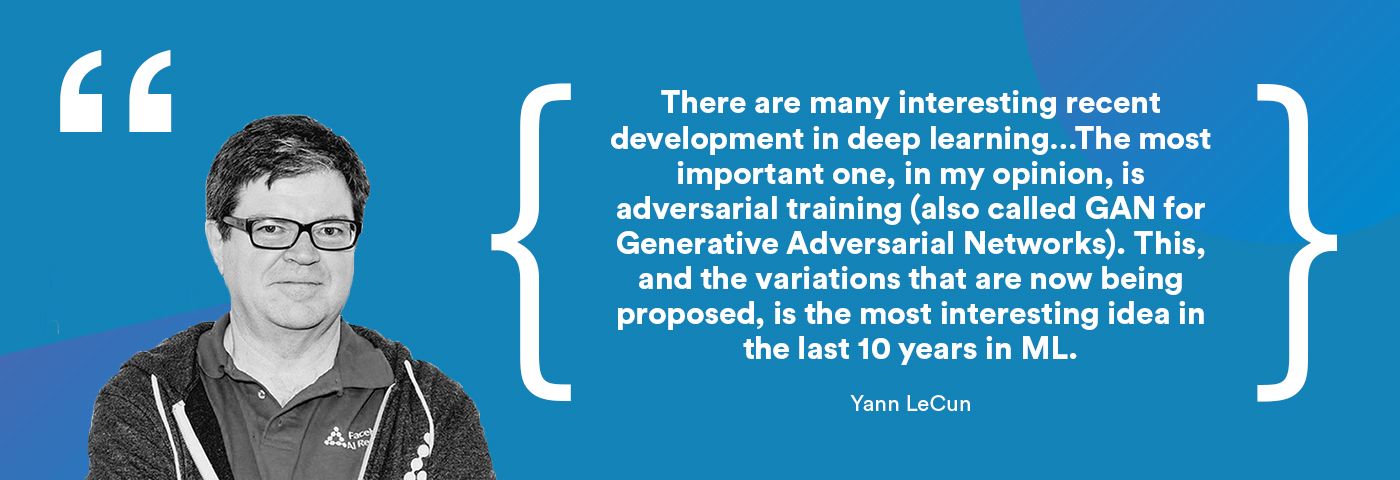
\includegraphics[width=\linewidth,keepaspectratio]{lecunn_quote}
\end{center}

\tiny{(Reference: Deep Learning basics - Rodrigo Agundez)}
\end{frame}



%%%%%%%%%%%%%%%%%%%%%%%%%%%%%%%%%%%%%%%%%%%%%%%%%%%
\begin{frame}[fragile] \frametitle{Why is DL useful?}
\begin{itemize}
\item ML features could be overspecified, incomplete and take long time to design
\item DL ``invents'' features.
\item Learned Features are easy to adapt, fast to learn
\item Deep learning provides a very flexible, (almost?) universal, learnable framework for representing world, visual and linguistic information
\end{itemize}
\end{frame}

%%%%%%%%%%%%%%%%%%%%%%%%%%%%%%%%%%%%%%%%%%%%%%%%%%%
\begin{frame}[fragile] \frametitle{Why is DL useful?}
\begin{itemize}
\item In ~2010 DL started outperforming other ML techniques 
\item First in speech and vision, then NLP
\end{itemize}
\begin{center}
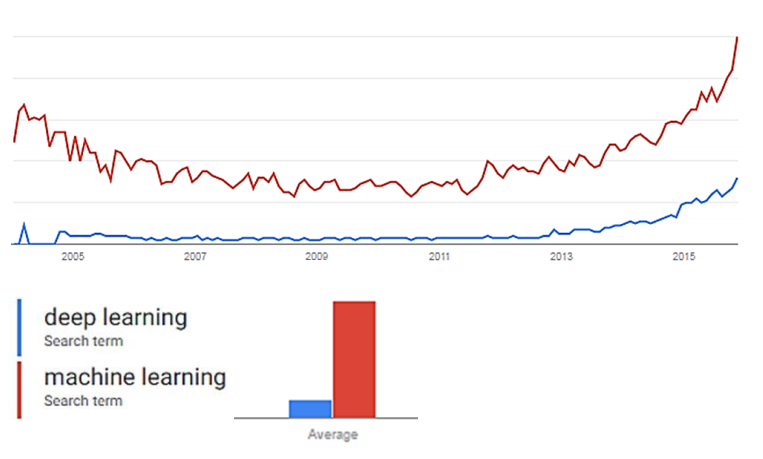
\includegraphics[width=\linewidth,keepaspectratio]{dl27}
\end{center}
\tiny{(Reference: Introduction to Deep Learning - Ismini Lourentzou)}
\end{frame}

%%%%%%%%%%%%%%%%%%%%%%%%%%%%%%%%%%%%%%%%%%%%%%%%%%%
\begin{frame}[fragile] \frametitle{Big Break-through in Vision}
\begin{center}
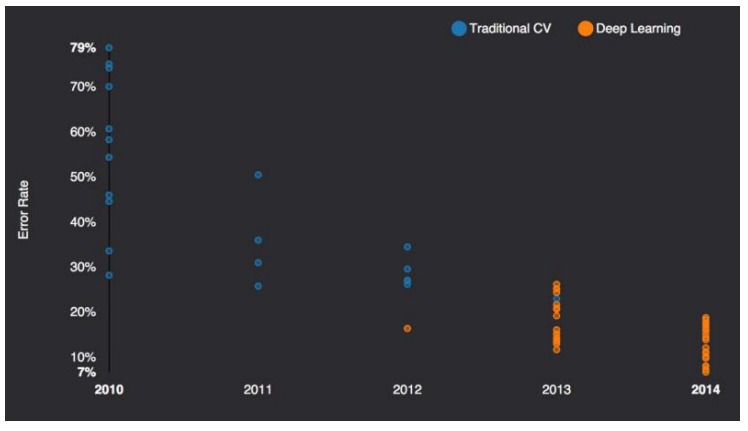
\includegraphics[width=0.8\linewidth,keepaspectratio]{ai38}
\end{center}
\tiny{(Reference: Introduction to Deep Learning - Ismini Lourentzou)}
\end{frame}

%%%%%%%%%%%%%%%%%%%%%%%%%%%%%%%%%%%%%%%%%%%%%%%%%%%
\begin{frame}[fragile] \frametitle{Big Break-through in Speech}
\begin{center}
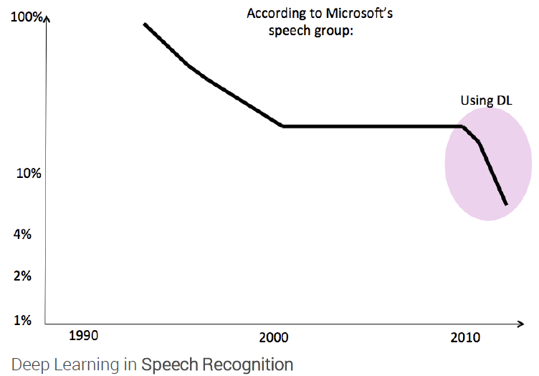
\includegraphics[width=0.8\linewidth,keepaspectratio]{ai51}
\end{center}
\tiny{(Reference: Introduction to Deep Learning - Ismini Lourentzou)}
\end{frame}

%%%%%%%%%%%%%%%%%%%%%%%%%%%%%%%%%%%%%%%%%%%%%%%%%%%
\begin{frame}[fragile] \frametitle{Deep Learning == Neural Nets }

\begin{itemize}
\item Main idea of deep learning: transform the input space into outputs via higher level abstractions.
\item Neural Net architectures are made up of perceptrons (similar to neurons) 
\item Each neuron carries certain transformations on inputs coming to it.
\item Collection of such neurons with various types of transformations, can create desired overall transformation.
\end{itemize}

\begin{center}
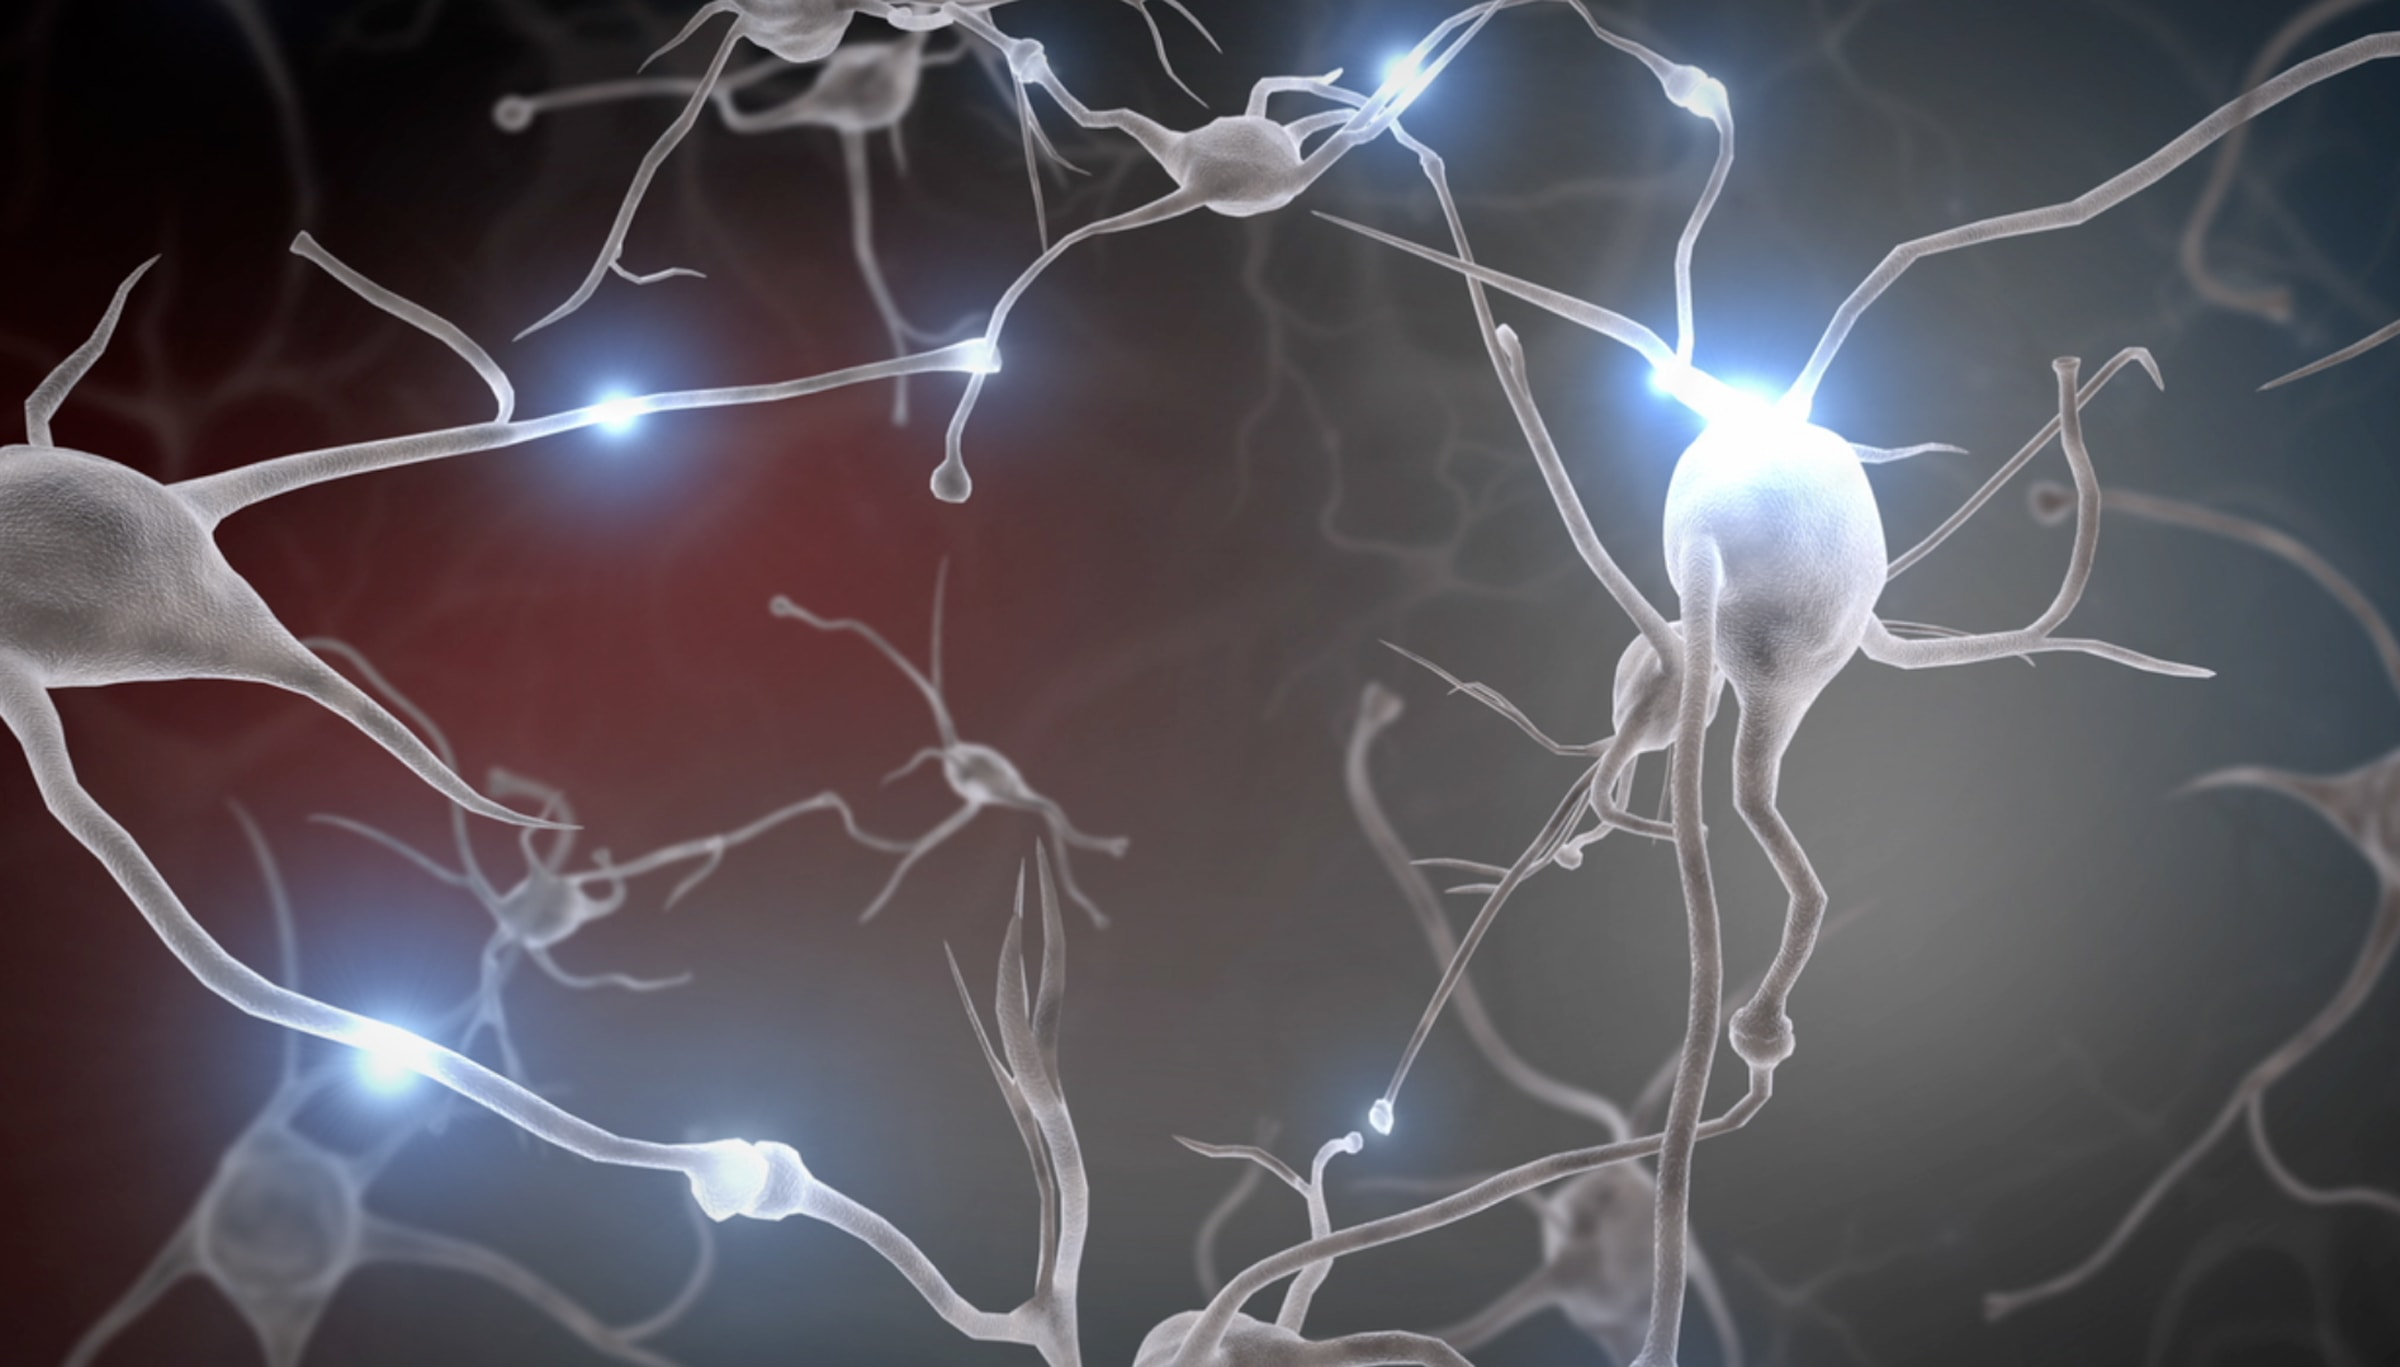
\includegraphics[width=0.4\linewidth,keepaspectratio]{neurons.jpg}
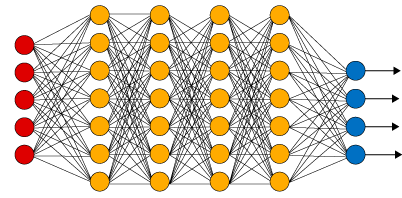
\includegraphics[width=0.4\linewidth,keepaspectratio]{dnn.png}
\end{center}

\tiny{(Reference: Deep Learning basics - Rodrigo Agundez)}

\end{frame}

%%%%%%%%%%%%%%%%%%%%%%%%%%%%%%%%%%%%%%%%%%%%%%%%%%%
\begin{frame}[fragile] \frametitle{Deep Learning == Neural Nets }
First artificial neuron proposed in 1943!

\begin{center}
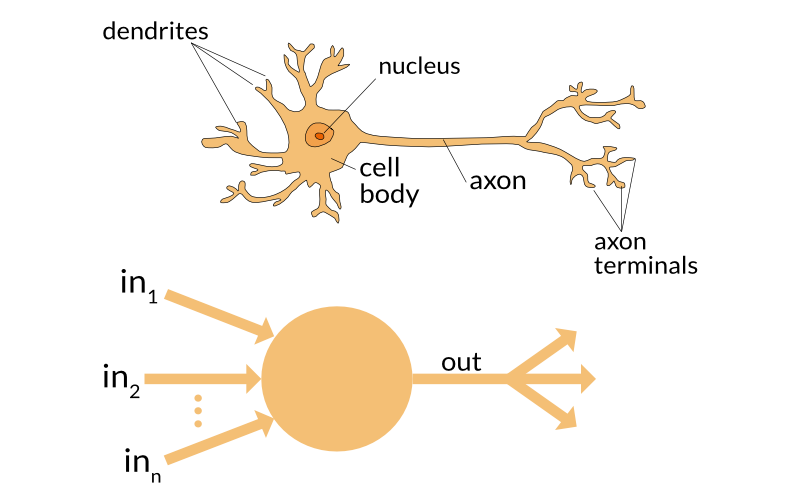
\includegraphics[width=\linewidth,keepaspectratio]{neuron_comparison.png}

\end{center}

\tiny{(Reference: Deep Learning basics - Rodrigo Agundez)}

\end{frame}


%%%%%%%%%%%%%%%%%%%%%%%%%%%%%%%%%%%%%%%%%%%%%%%%%%%
\begin{frame}[fragile] \frametitle{Artificial neuron}

\begin{center}
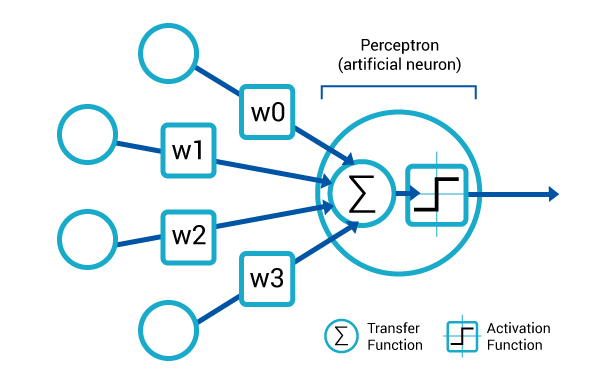
\includegraphics[width=\linewidth,keepaspectratio]{artificial_neuron.jpg}

\end{center}

\tiny{(Reference: Deep Learning basics - Rodrigo Agundez)}

\end{frame}

%%%%%%%%%%%%%%%%%%%%%%%%%%%%%%%%%%%%%%%%%%%%%%%%%%%
\begin{frame}[fragile] \frametitle{Layers}

Hierarchical feature representations

\begin{center}
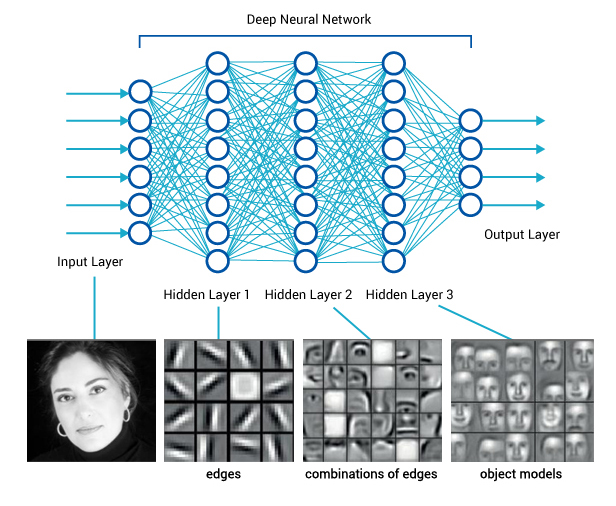
\includegraphics[width=0.7\linewidth,keepaspectratio]{layers.jpg}

\end{center}

\tiny{(Reference: Deep Learning basics - Rodrigo Agundez)}

\end{frame}

%%%%%%%%%%%%%%%%%%%%%%%%%%%%%%%%%%%%%%%%%%%%%%%%%%%
\begin{frame}[fragile] \frametitle{Neural Networks}

\begin{center}
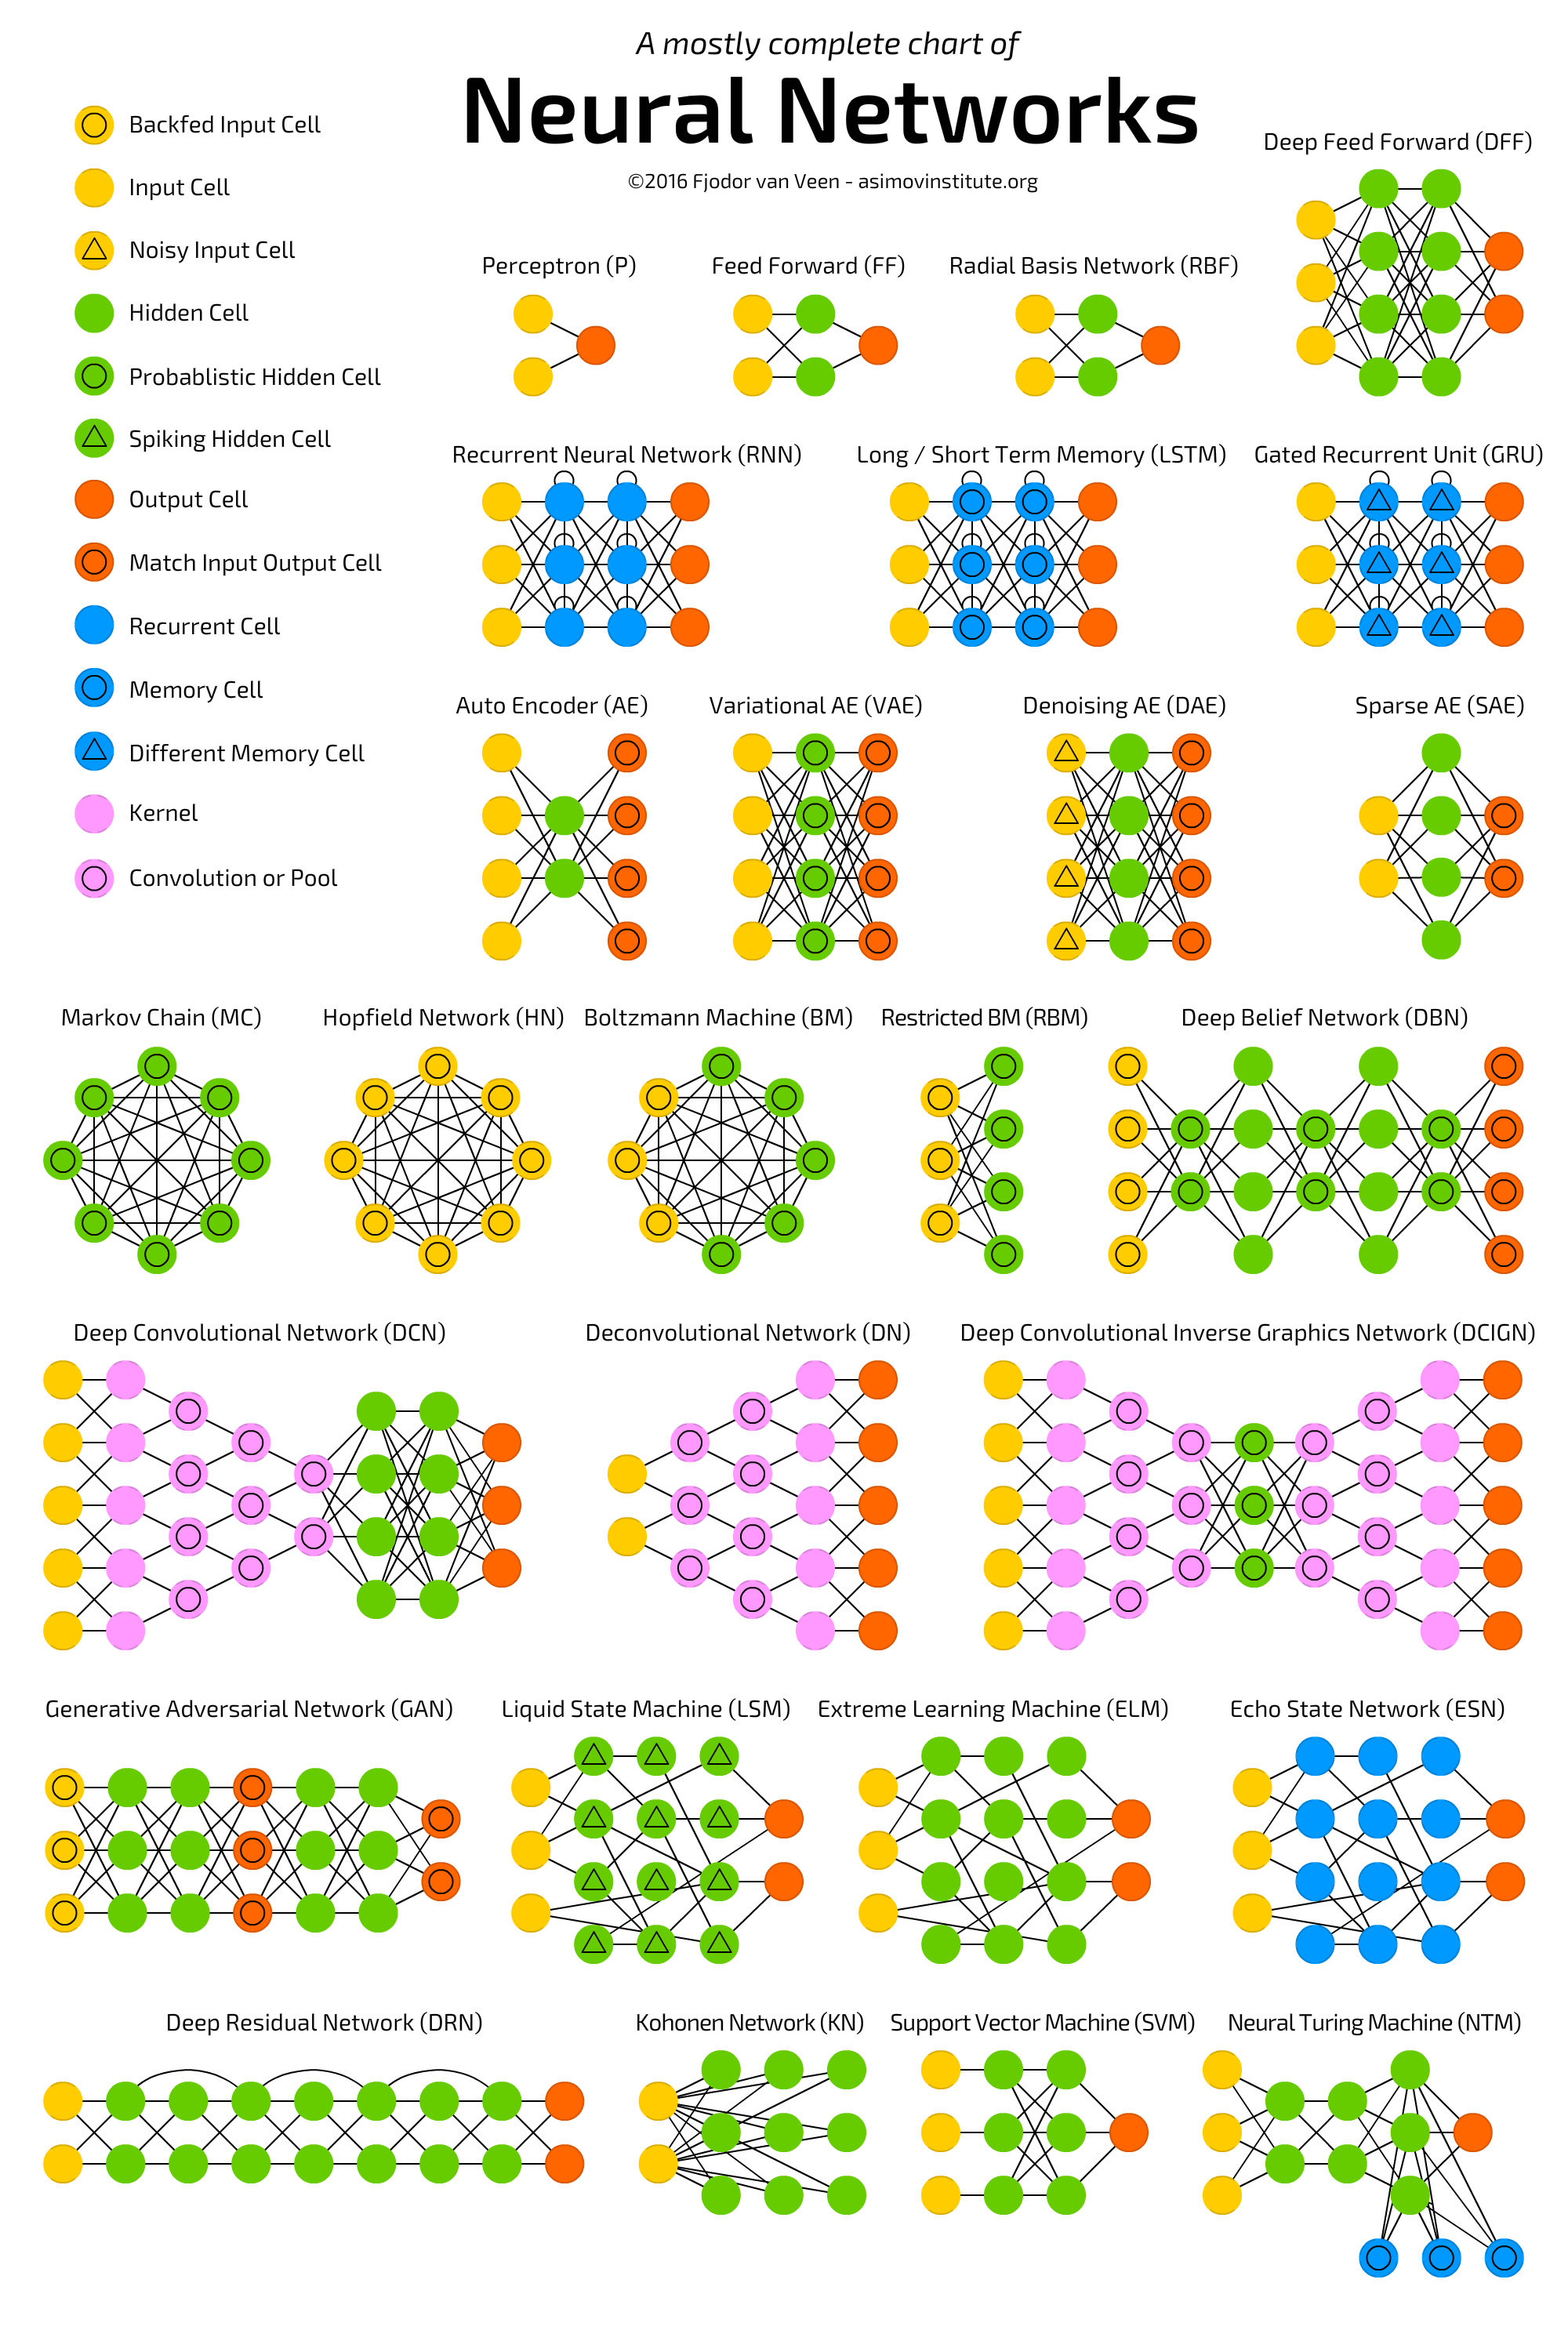
\includegraphics[width=0.4\linewidth,keepaspectratio]{neural_networks_collection.png}

\end{center}

\tiny{(Reference: Deep Learning basics - Rodrigo Agundez)}

\end{frame}


%%%%%%%%%%%%%%%%%%%%%%%%%%%%%%%%%%%%%%%%%%%%%%%%%%%%%%%%%%%%%%%%%%%%%%%%%%%%%%%%%%
\begin{frame}[fragile]\frametitle{}
\begin{center}
{\Large Neural Networks Training Process: Non Mathematical}
\end{center}
\end{frame}



% %%%%%%%%%%%%%%%%%%%%%%%%%%%%%%%%%%%%%%%%%%%%%%%%%%%
% \begin{frame}[fragile] \frametitle{Structure}
% \begin{center}
% 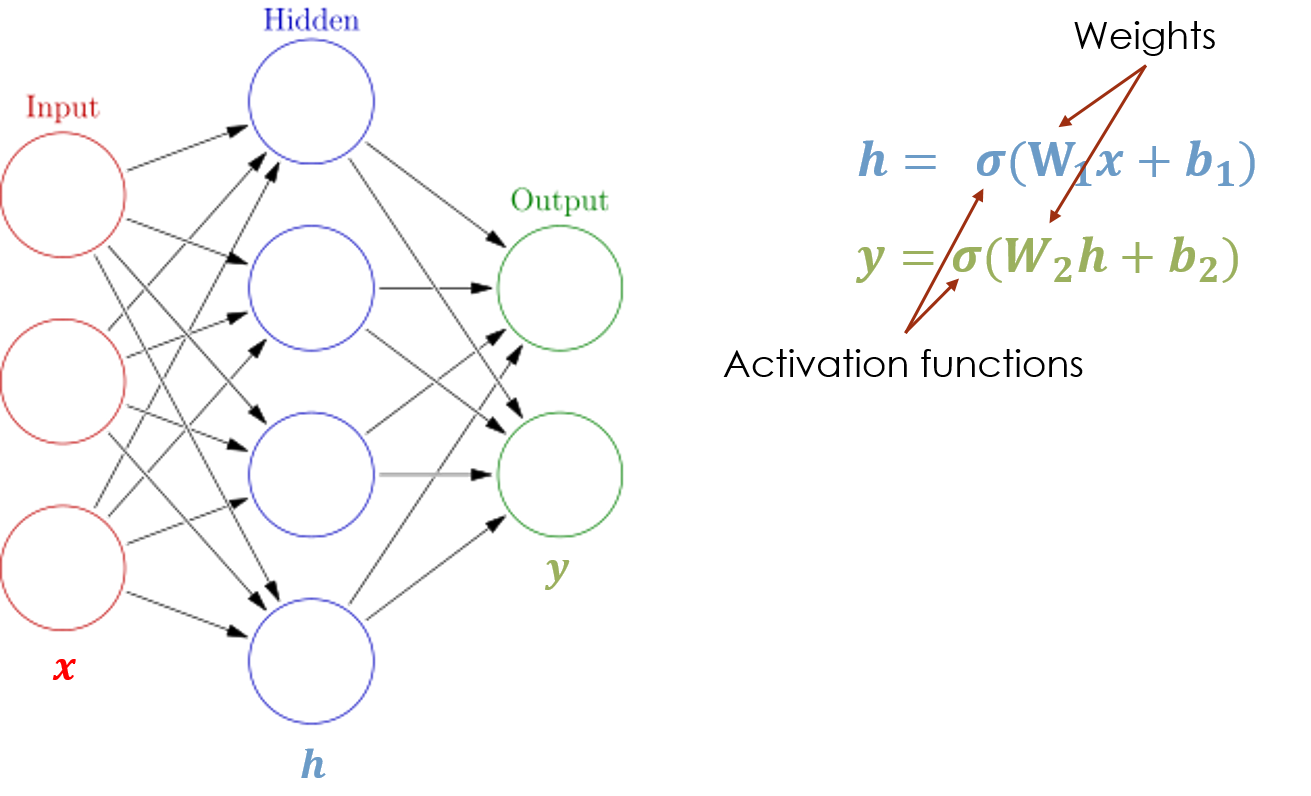
\includegraphics[width=\linewidth,keepaspectratio]{ai52}
% \end{center}
% \tiny{(Reference: Introduction to Deep Learning - Ismini Lourentzou)}
% \end{frame}

%%%%%%%%%%%%%%%%%%%%%%%%%%%%%%%%%%%%%%%%%%%%%%%%%%%
\begin{frame}[fragile] \frametitle{Training Process: Non Mathematical}
\begin{center}
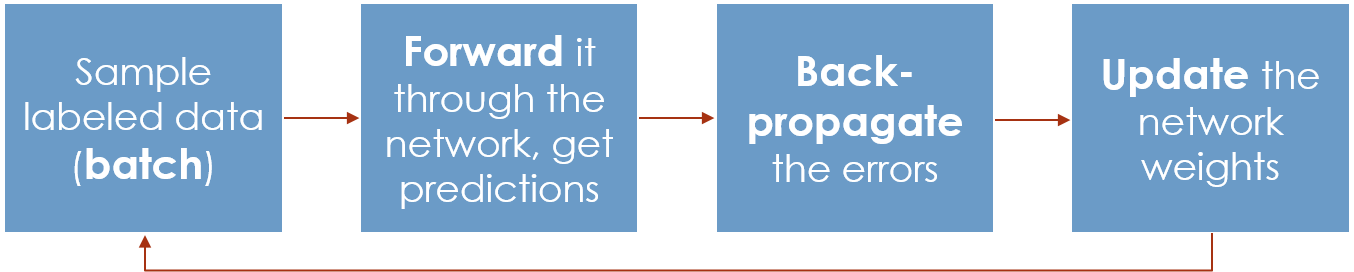
\includegraphics[width=\linewidth,keepaspectratio]{ai53}
\end{center}
\tiny{(Reference: Introduction to Deep Learning - Ismini Lourentzou)}
\end{frame}




%%%%%%%%%%%%%%%%%%%%%%%%%%%%%%%%%%%%%%%%%%%%%%%%%%%
\begin{frame}[fragile] \frametitle{Data Enters }
\begin{center}
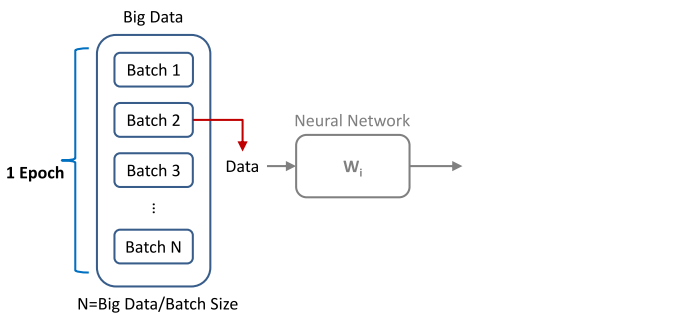
\includegraphics[width=\linewidth,keepaspectratio]{nnb1}
\end{center}
\tiny{(Reference:PyTorch Tutorial-NTU Machine Learning Course-Lyman Lin )}
\end{frame}

%%%%%%%%%%%%%%%%%%%%%%%%%%%%%%%%%%%%%%%%%%%%%%%%%%%
\begin{frame}[fragile] \frametitle{Forward Pass}
\begin{center}
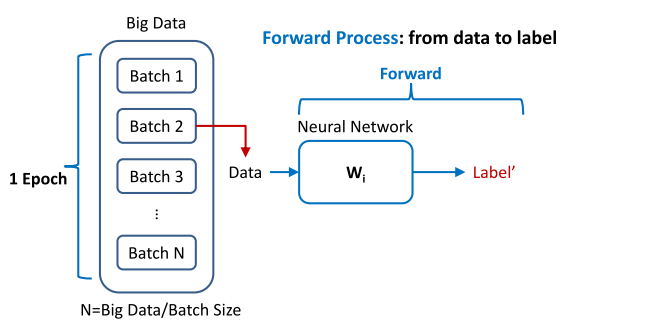
\includegraphics[width=\linewidth,keepaspectratio]{nnb2}
\end{center}
\tiny{(Reference:PyTorch Tutorial-NTU Machine Learning Course-Lyman Lin )}
\end{frame}
%%%%%%%%%%%%%%%%%%%%%%%%%%%%%%%%%%%%%%%%%%%%%%%%%%%
\begin{frame}[fragile] \frametitle{Loss Calculations}
\begin{center}
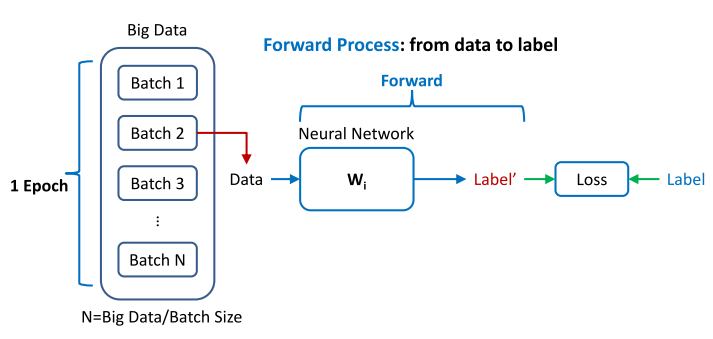
\includegraphics[width=\linewidth,keepaspectratio]{nnb3}
\end{center}
\tiny{(Reference:PyTorch Tutorial-NTU Machine Learning Course-Lyman Lin )}
\end{frame}
%%%%%%%%%%%%%%%%%%%%%%%%%%%%%%%%%%%%%%%%%%%%%%%%%%%
\begin{frame}[fragile] \frametitle{Back Propagation}
\begin{center}
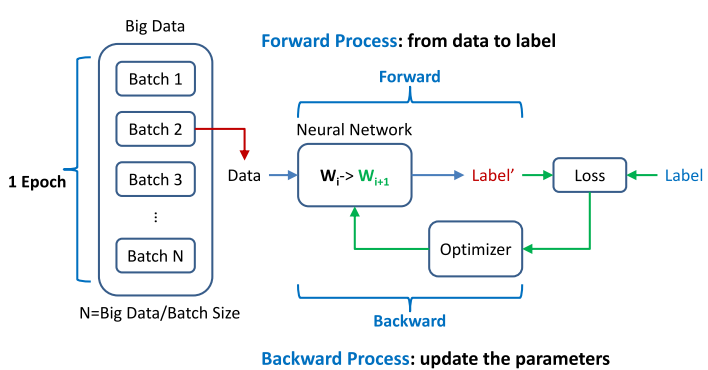
\includegraphics[width=\linewidth,keepaspectratio]{nnb4}
\end{center}
\tiny{(Reference:PyTorch Tutorial-NTU Machine Learning Course-Lyman Lin )}
\end{frame}
%%%%%%%%%%%%%%%%%%%%%%%%%%%%%%%%%%%%%%%%%%%%%%%%%%%
\begin{frame}[fragile] \frametitle{Overall Process}
\begin{center}
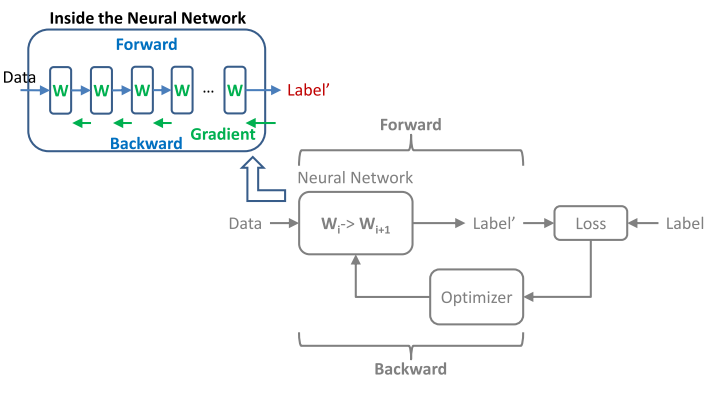
\includegraphics[width=\linewidth,keepaspectratio]{nnb5}
\end{center}
\tiny{(Reference:PyTorch Tutorial-NTU Machine Learning Course-Lyman Lin )}
\end{frame}
% %%%%%%%%%%%%%%%%%%%%%%%%%%%%%%%%%%%%%%%%%%%%%%%%%%%
% \begin{frame}[fragile] \frametitle{Data Flow}
% \begin{center}
% 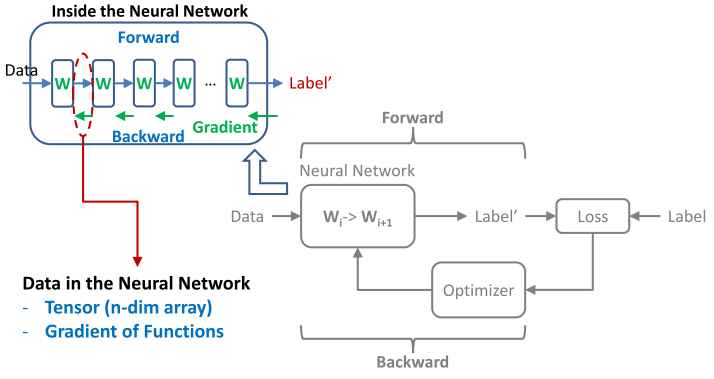
\includegraphics[width=\linewidth,keepaspectratio]{nnb6}
% \end{center}
% \tiny{(Reference:PyTorch Tutorial-NTU Machine Learning Course-Lyman Lin )}
% \end{frame}



% %%%%%%%%%%%%%%%%%%%%%%%%%%%%%%%%%%%%%%%%%%%%%%%%%%%
% \begin{frame}[fragile] \frametitle{Forward Pass }
% \begin{center}
% 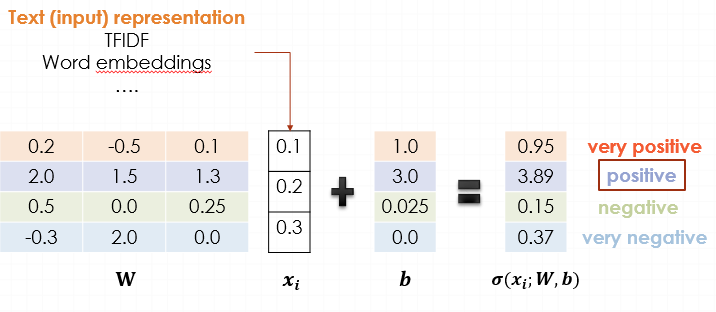
\includegraphics[width=\linewidth,keepaspectratio]{ai56}
% \end{center}
% \tiny{(Reference: Introduction to Deep Learning - Ismini Lourentzou)}
% \end{frame}

% %%%%%%%%%%%%%%%%%%%%%%%%%%%%%%%%%%%%%%%%%%%%%%%%%%%%%%%%%%%%%%%%%%%%%%%%%%%%%%%%%%
% \begin{frame}[fragile]\frametitle{}
% \begin{center}
% {\Large Types of Networks}
% \end{center}
% \end{frame}



% %%%%%%%%%%%%%%%%%%%%%%%%%%%%%%%%%%%%%%%%%%%%%%%%%%%
% \begin{frame}[fragile] \frametitle{CNN}
% Main CNN idea for text: Compute vectors for n-grams and group them afterwards
% \begin{center}
% 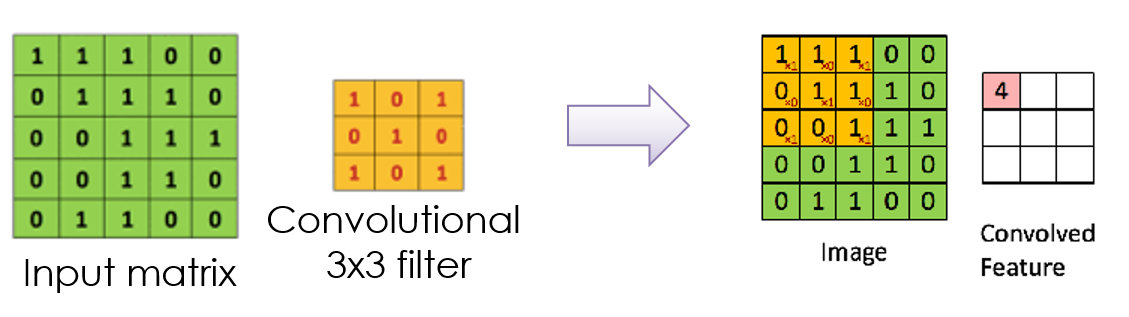
\includegraphics[width=\linewidth,keepaspectratio]{cnntxt}
% \end{center}
% \tiny{(Reference: http://deeplearning.stanford.edu/wiki/index.php/Feature\_extraction\_using\_convolution)}
% \end{frame}

% %%%%%%%%%%%%%%%%%%%%%%%%%%%%%%%%%%%%%%%%%%%%%%%%%%%
% \begin{frame}[fragile] \frametitle{CNN}
% Twitter Sentiment Classification
% \begin{center}
% 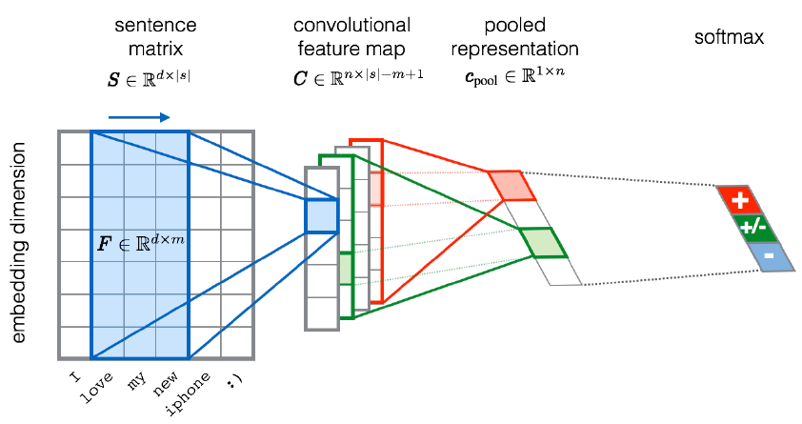
\includegraphics[width=\linewidth,keepaspectratio]{cnnsent}
% \end{center}
% \tiny{(Reference: Severyn, Aliaksei, and Alessandro Moschitti. "UNITN: Training Deep Convolution Neural Network for Twitter Sentiment Classification." SemEval@ NAACL-HLT. 2015.
% )}
% \end{frame}

% %%%%%%%%%%%%%%%%%%%%%%%%%%%%%%%%%%%%%%%%%%%%%%%%%%%
% \begin{frame}[fragile] \frametitle{RNN}
% Main RNN idea for text: Condition on all previous words. Use same set of weights at all time steps

% \begin{center}
% 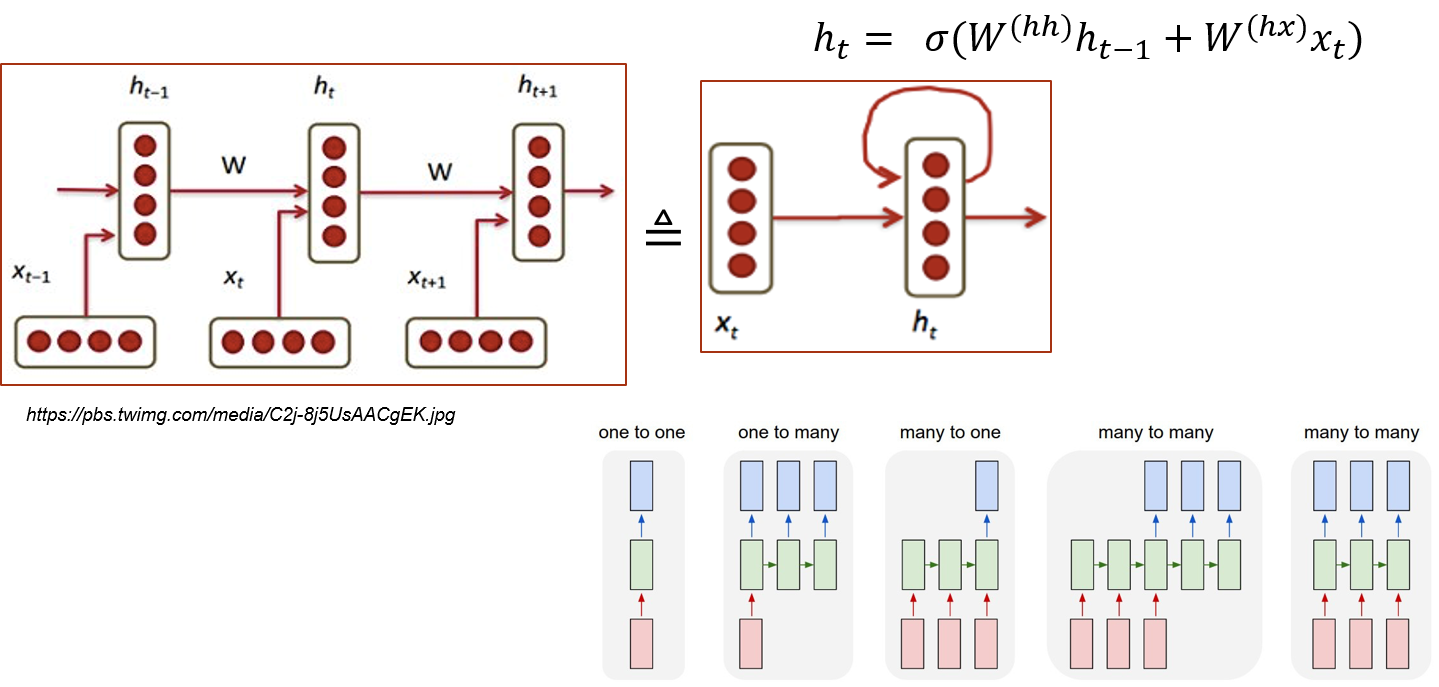
\includegraphics[width=\linewidth,keepaspectratio]{rnn25}
% \end{center}
% \tiny{(Reference: https://discuss.pytorch.org/uploads/default/original/1X/6415da0424dd66f2f5b134709b92baa59e604c55.jpg)}
% \end{frame}


% %%%%%%%%%%%%%%%%%%%%%%%%%%%%%%%%%%%%%%%%%%%%%%%%%%%
% \begin{frame}[fragile] \frametitle{RNN}
% Main idea: incorporate both left and right context
% output may not only depend on the previous elements in the sequence,  but also future elements. 
% \begin{center}
% 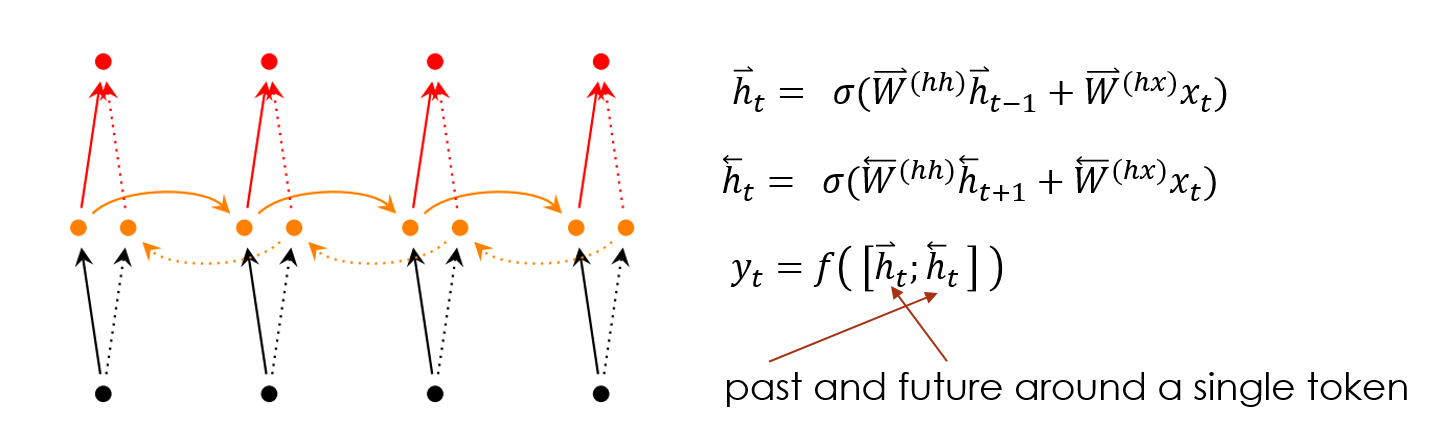
\includegraphics[width=\linewidth,keepaspectratio]{rnn26}
% \end{center}
% Two RNNs stacked on top of each other. Output is computed based on the hidden state of both RNNs 
% \tiny{(Reference: http://www.wildml.com/2015/09/recurrent-neural-networks-tutorial-part-1-introduction-to-rnns/)}
% \end{frame}

% %%%%%%%%%%%%%%%%%%%%%%%%%%%%%%%%%%%%%%%%%%%%%%%%%%%
% \begin{frame}[fragile] \frametitle{Seq2seq}
% \begin{center}
% 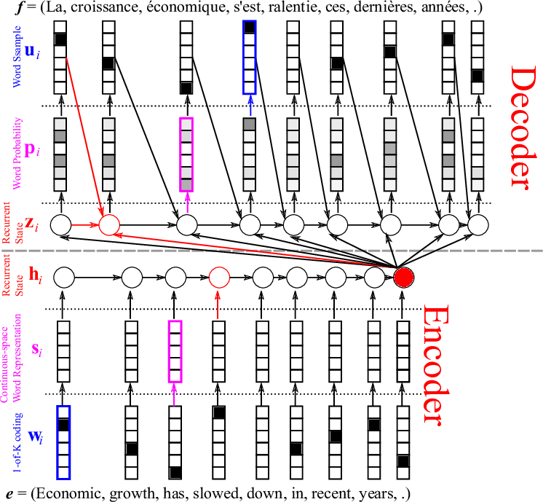
\includegraphics[width=0.6\linewidth,keepaspectratio]{rnn27}
% \end{center}
% \tiny{(Reference: Cho, Kyunghyun, et al. ``Learning phrase representations using RNN encoder-decoder for statistical machine translation.'' EMNLP 2014)}
% \end{frame}


% %%%%%%%%%%%%%%%%%%%%%%%%%%%%%%%%%%%%%%%%%%%%%%%%%%%
% \begin{frame}[fragile] \frametitle{Seq2seq}
% Application Example: Relation Extraction from text
% \begin{center}
% 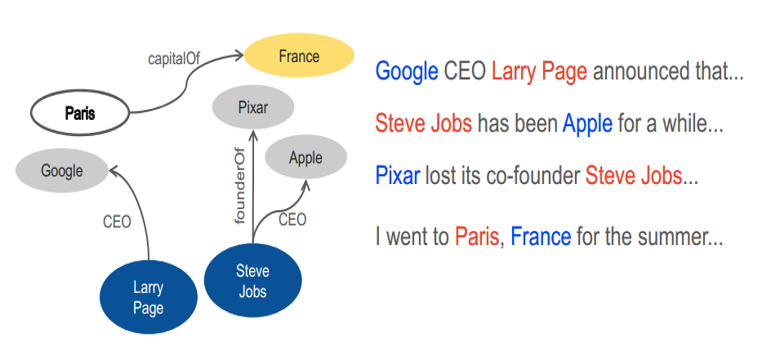
\includegraphics[width=\linewidth,keepaspectratio]{dl31}
% \end{center}
% \tiny{(Reference: http://www.mathcs.emory.edu/~dsavenk/slides/relation\_extraction/img/distant.png)}
% \end{frame}


% %%%%%%%%%%%%%%%%%%%%%%%%%%%%%%%%%%%%%%%%%%%%%%%%%%%
% \begin{frame}[fragile] \frametitle{Task: binary (or multi-class) classification  }
% \begin{itemize}
% \item  Sentence $S = w_1 w_2 .. e_1 .. w_j .. e_2 .. w_n$ where  $e_1$ and $e_2$ entities.
% \item ``The new {\bf iPhone 7 Plus} includes an improved {\bf camera} to take amazing pictures.''
% \item  $Component-Whole(e_1 , e_2 )$ ? YES / NO
% \end{itemize}
% \end{frame}

% %%%%%%%%%%%%%%%%%%%%%%%%%%%%%%%%%%%%%%%%%%%%%%%%%%%
% \begin{frame}[fragile] \frametitle{Input representation}
% \begin{center}
% 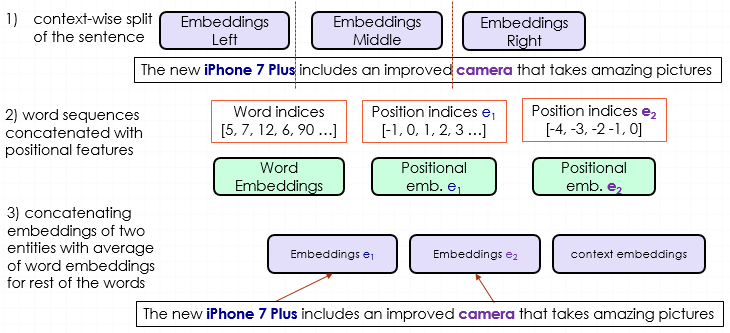
\includegraphics[width=\linewidth,keepaspectratio]{ai59}
% \end{center}
% \tiny{(Reference: Introduction to Deep Learning - Ismini Lourentzou)}
% \end{frame}

% %%%%%%%%%%%%%%%%%%%%%%%%%%%%%%%%%%%%%%%%%%%%%%%%%%%
% \begin{frame}[fragile] \frametitle{Models: MLP}
% Simple fully-connected multi-layer perceptron
% \begin{center}
% 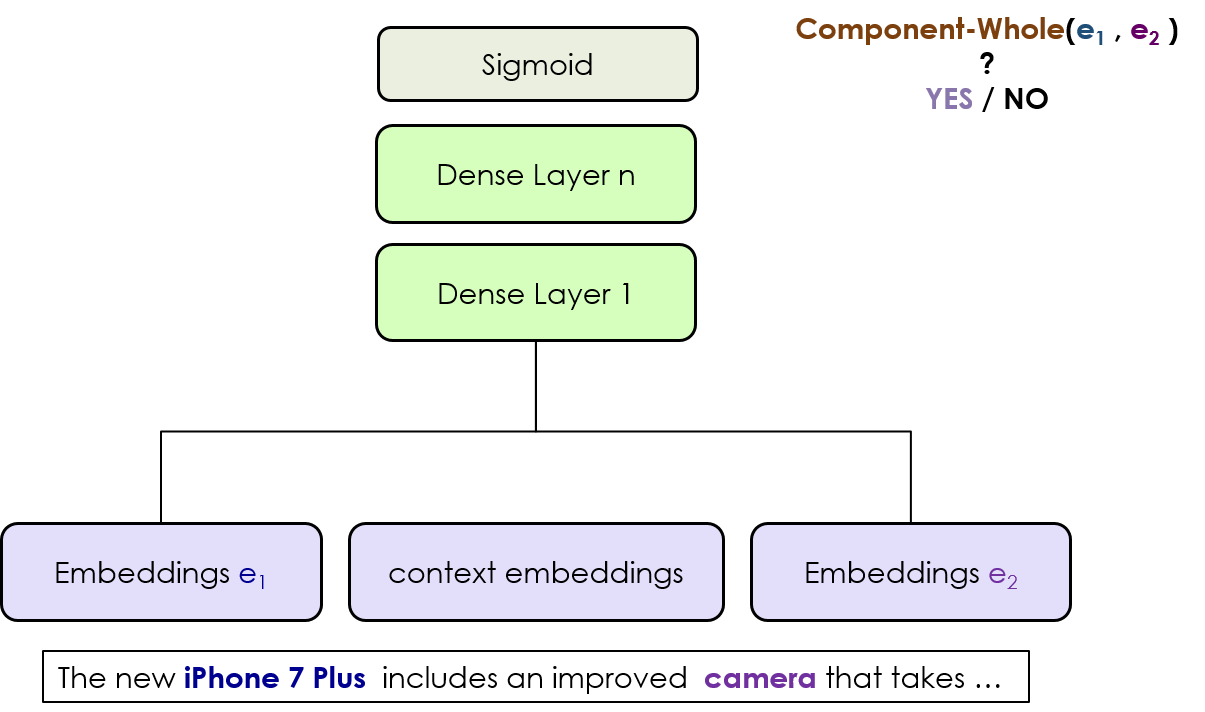
\includegraphics[width=\linewidth,keepaspectratio]{ai61}
% \end{center}
% \tiny{(Reference: Introduction to Deep Learning - Ismini Lourentzou)}
% \end{frame}

% %%%%%%%%%%%%%%%%%%%%%%%%%%%%%%%%%%%%%%%%%%%%%%%%%%%
% \begin{frame}[fragile] \frametitle{Models: CNN}
% \begin{center}
% 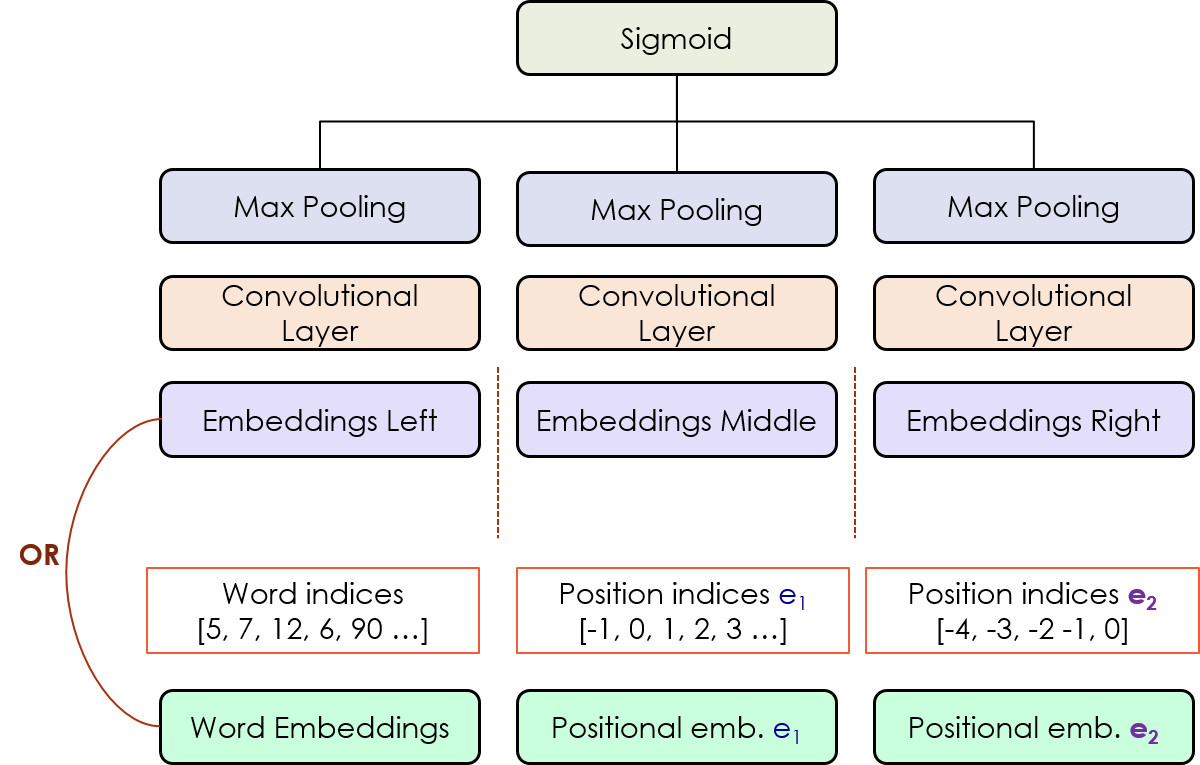
\includegraphics[width=\linewidth,keepaspectratio]{ai62}
% \end{center}
% \tiny{(Reference: Zeng, D.et al. “Relation classification via convolution deep neural network”.COLING (2014))}
% \end{frame}

% %%%%%%%%%%%%%%%%%%%%%%%%%%%%%%%%%%%%%%%%%%%%%%%%%%%
% \begin{frame}[fragile] \frametitle{Models: CNN}
% \begin{center}
% 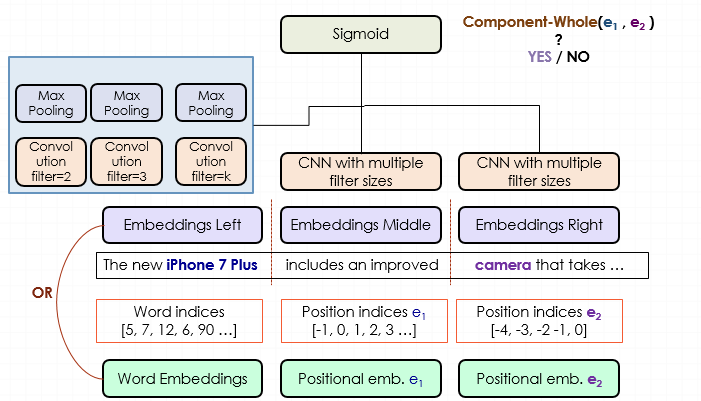
\includegraphics[width=\linewidth,keepaspectratio]{ai63}
% \end{center}
% \tiny{(Reference: Nguyen, T.H., Grishman, R. ``Relation extraction: Perspective from convolution neural networks.'' VS@ HLT-NAACL. (2015))}
% \end{frame}

%%%%%%%%%%%%%%%%%%%%%%%%%%%%%%%%%%%%%%%%%%%%%%%%%%%%%%%%%%%%%%%%%%%%%%%%%%%%%%%%%%
\begin{frame}[fragile]\frametitle{}
\begin{center}
{\Large Neural Networks Training Process: Mathematical}
\end{center}
\end{frame}

%%%%%%%%%%%%%%%%%%%%%%%%%%%%%%%%%%%%%%%%%%%%%%%%%%%
\begin{frame}[fragile] \frametitle{Start}

\begin{center}
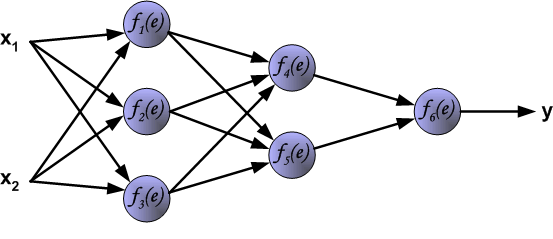
\includegraphics[width=0.8\linewidth,keepaspectratio]{model_diagram}

\end{center}

\tiny{(Reference: Deep Learning basics - Rodrigo Agundez)}

\end{frame}


%%%%%%%%%%%%%%%%%%%%%%%%%%%%%%%%%%%%%%%%%%%%%%%%%%%
\begin{frame}[fragile] \frametitle{Forward pass}

\begin{center}
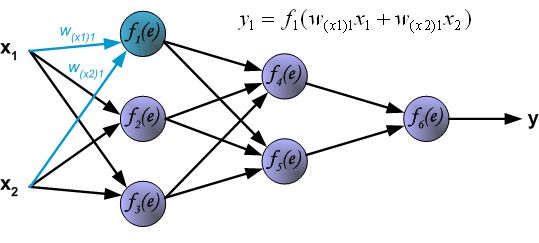
\includegraphics[width=0.8\linewidth,keepaspectratio]{forward_pass_0}

\end{center}

\tiny{(Reference: Deep Learning basics - Rodrigo Agundez)}

\end{frame}

%%%%%%%%%%%%%%%%%%%%%%%%%%%%%%%%%%%%%%%%%%%%%%%%%%%
\begin{frame}[fragile] \frametitle{Forward pass}

\begin{center}
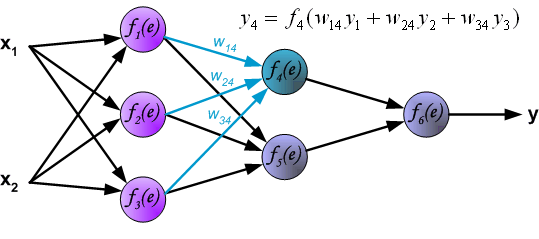
\includegraphics[width=0.8\linewidth,keepaspectratio]{forward_pass_1}

\end{center}

\tiny{(Reference: Deep Learning basics - Rodrigo Agundez)}

\end{frame}

%%%%%%%%%%%%%%%%%%%%%%%%%%%%%%%%%%%%%%%%%%%%%%%%%%%
\begin{frame}[fragile] \frametitle{Forward pass}

\begin{center}
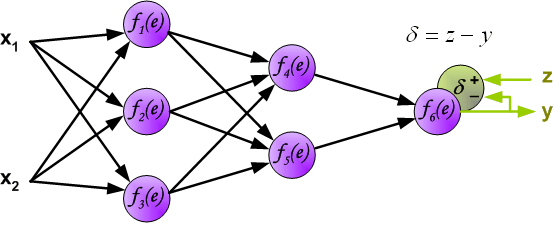
\includegraphics[width=0.8\linewidth,keepaspectratio]{forward_pass_2}

\end{center}

\tiny{(Reference: Deep Learning basics - Rodrigo Agundez)}

\end{frame}

%%%%%%%%%%%%%%%%%%%%%%%%%%%%%%%%%%%%%%%%%%%%%%%%%%%
\begin{frame}[fragile] \frametitle{Backpropagation}

\begin{center}
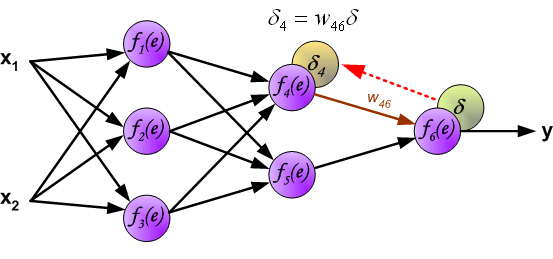
\includegraphics[width=0.8\linewidth,keepaspectratio]{backpropagation_0}

\end{center}

\tiny{(Reference: Deep Learning basics - Rodrigo Agundez)}

\end{frame}

%%%%%%%%%%%%%%%%%%%%%%%%%%%%%%%%%%%%%%%%%%%%%%%%%%%
\begin{frame}[fragile] \frametitle{Backpropagation}

\begin{center}
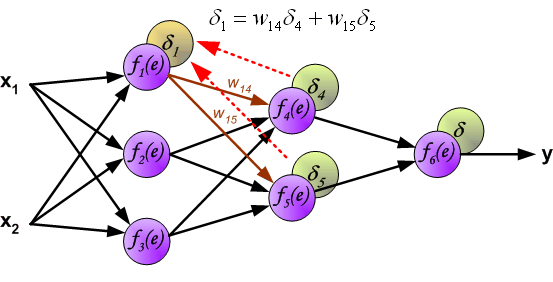
\includegraphics[width=0.8\linewidth,keepaspectratio]{backpropagation_1}

\end{center}

\tiny{(Reference: Deep Learning basics - Rodrigo Agundez)}

\end{frame}

%%%%%%%%%%%%%%%%%%%%%%%%%%%%%%%%%%%%%%%%%%%%%%%%%%%
\begin{frame}[fragile] \frametitle{Backpropagation}

\begin{center}
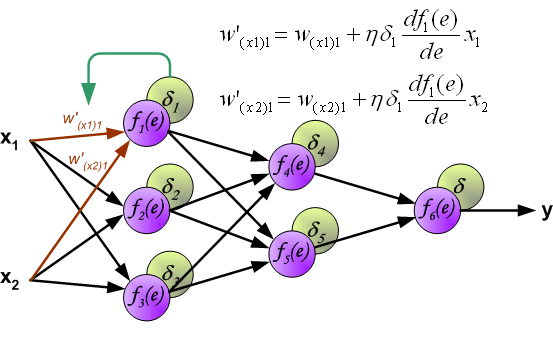
\includegraphics[width=0.8\linewidth,keepaspectratio]{backpropagation_2}

\end{center}

\tiny{(Reference: Deep Learning basics - Rodrigo Agundez)}

\end{frame}

%%%%%%%%%%%%%%%%%%%%%%%%%%%%%%%%%%%%%%%%%%%%%%%%%%%
\begin{frame}[fragile] \frametitle{Backpropagation}

\begin{center}
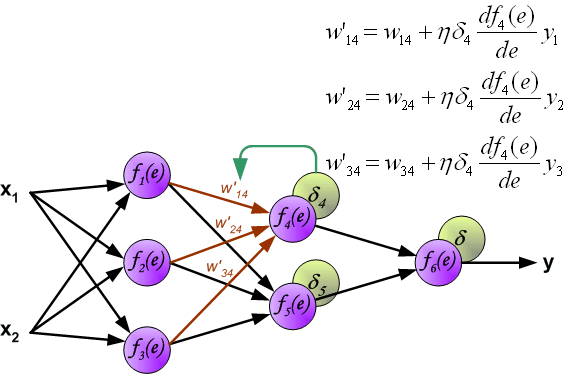
\includegraphics[width=0.8\linewidth,keepaspectratio]{backpropagation_3}

\end{center}

\tiny{(Reference: Deep Learning basics - Rodrigo Agundez)}

\end{frame}

%%%%%%%%%%%%%%%%%%%%%%%%%%%%%%%%%%%%%%%%%%%%%%%%%%%
\begin{frame}[fragile] \frametitle{Backpropagation}


\begin{itemize}
\item Starts at the end of the net and tunes each layer using the gradient of the loss function. Repeatedly applies the chain rule. 

\item Numeric approximation: $f'(x) \approx \frac{f(x+h) - f(x)}{h}$

\item Symbolic differentiation: Symbolic, exact representation of the derivative.

\item Reverse automatic differentiation
\end{itemize}


\begin{center}
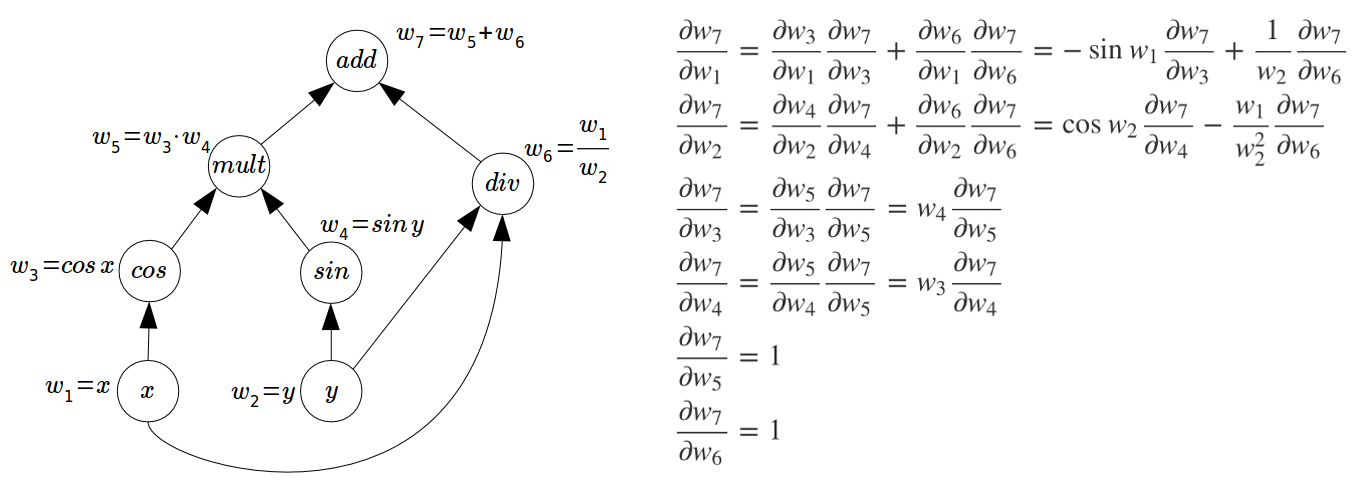
\includegraphics[width=0.8\linewidth,keepaspectratio]{automatic-differentiation}
\end{center}

\tiny{(Reference: Deep Learning basics - Rodrigo Agundez)}

\end{frame}

%%%%%%%%%%%%%%%%%%%%%%%%%%%%%%%%%%%%%%%%%%%%%%%%%%%
\begin{frame}[fragile] \frametitle{Optimization by backpropagation}
\begin{itemize}
\item Loss/cost function
\item Gradient descent
\end{itemize}

\begin{center}
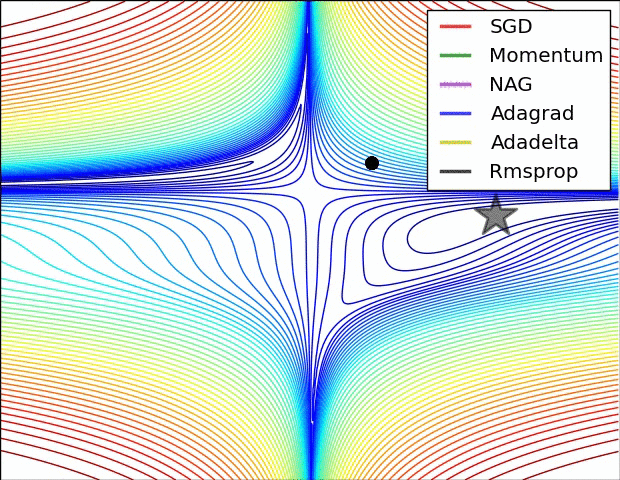
\includegraphics[width=0.4\linewidth,keepaspectratio]{optimizers_1}
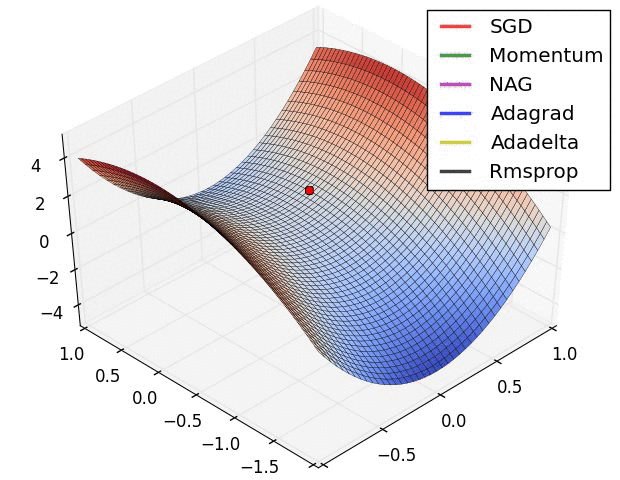
\includegraphics[width=0.4\linewidth,keepaspectratio]{optimizers_2}
\end{center}

\tiny{(Reference: Deep Learning basics - Rodrigo Agundez)}

\end{frame}

%%%%%%%%%%%%%%%%%%%%%%%%%%%%%%%%%%%%%%%%%%%%%%%%%%%%%%%%%%%%%%%%%%%%%%%%%%%%%%%%%%
\begin{frame}[fragile]\frametitle{}
\begin{center}
{\Large Other Aspects}
\end{center}
\end{frame}

%%%%%%%%%%%%%%%%%%%%%%%%%%%%%%%%%%%%%%%%%%%%%%%%%%%
\begin{frame}[fragile] \frametitle{Challenges of Deep Learning}
\begin{itemize}
\item Explain-ability - How do you learn what you learn?
\item Debugging - What has gone wrong?
\item Why is this not converging?
\end{itemize}
\tiny{(Reference: AI and Deep Learning - Subrat Panda)}
\end{frame}

%%%%%%%%%%%%%%%%%%%%%%%%%%%%%%%%%%%%%%%%%%%%%%%%%%%%%%%%%%%%%%%%%%%%%%%%%%%%%%%%%%
\begin{frame}[fragile]\frametitle{Usage Requirements}
\begin{itemize}
\item Large data set with good quality (input-output mappings)
\item Measurable and describable goals (define the cost)
\item Enough computing power (AWS GPU Instance)
\item Excels in tasks where the basic unit (pixel, word) has very little
meaning in itself, but the combination of such units has a useful
meaning.
\end{itemize}
{\tiny (Deep Learning - The Past, Present and Future of Artificial Intelligence - Lukas Masuch)}
\end{frame}


%%%%%%%%%%%%%%%%%%%%%%%%%%%%%%%%%%%%%%%%%%%%%%%%%%%
\begin{frame}[fragile] \frametitle{Deep Learning Tools}
\begin{center}
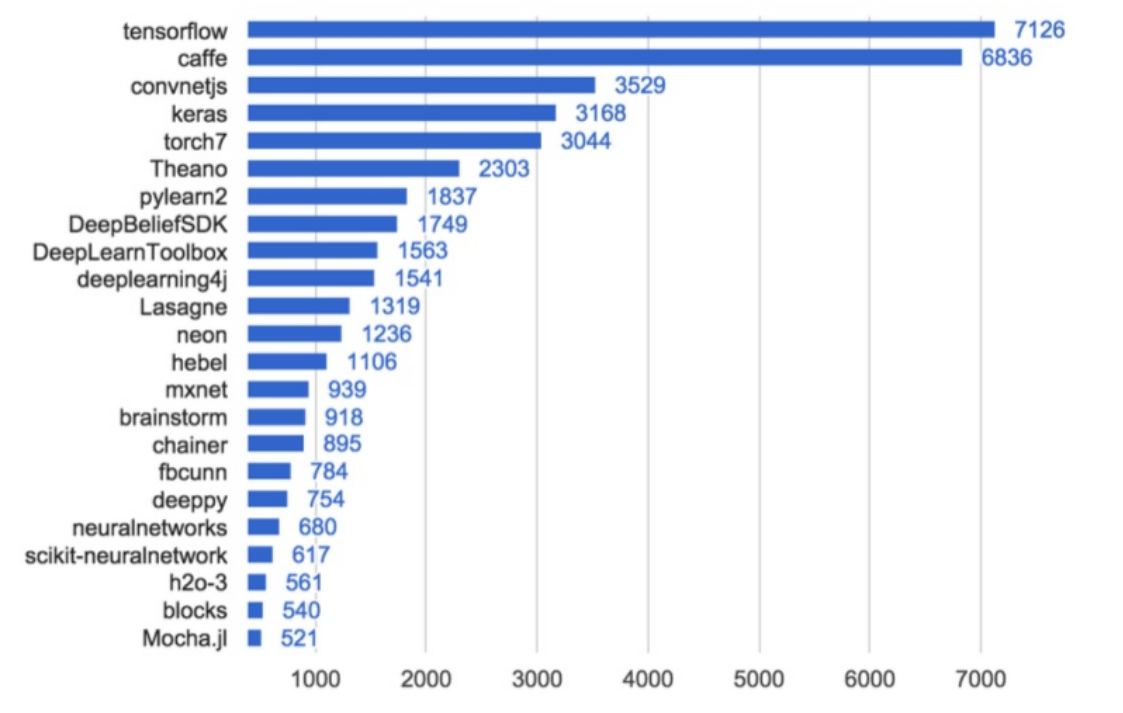
\includegraphics[width=0.8\linewidth,keepaspectratio]{dl32}
\end{center}
\tiny{(Reference: Introduction to Deep Learning - Ismini Lourentzou)}
\end{frame}

%%%%%%%%%%%%%%%%%%%%%%%%%%%%%%%%%%%%%%%%%%%%%%%%%%%
\begin{frame}[fragile] \frametitle{Deep Learning Outlook}
\begin{itemize}
\item Significant advances in deep reinforcement and unsupervised learning
\item Bigger and more complex architectures
\item Harder problems being attempted
\end{itemize}
\end{frame}



